% ===========================================================================
% OmicsCouncil — Springer LNCS manuscript. Compile with pdflatex + bibtex (splncs04).
%
% NOTE ON NUMBERS: cells marked with \tbd are placeholders to be filled from
% the JSON written by scripts/run_all.sh (results/*.json). They are kept
% explicit on purpose so no value is ever invented in the manuscript.
%
% NOTE ON ANONYMITY: for double-blind review, comment out the \author /
% \institute block and use the anonymous one provided below.
% ===========================================================================
\documentclass[runningheads]{llncs}

\usepackage[T1]{fontenc}
\usepackage[utf8]{inputenc}
\usepackage{graphicx}
\usepackage{amsmath,amssymb}
\usepackage{booktabs}
\usepackage{xcolor}
\usepackage{hyperref}
\usepackage{tikz}
\usetikzlibrary{positioning,arrows.meta,fit,backgrounds}

% Placeholder marker for not-yet-computed numbers.
\newcommand{\tbd}{\textcolor{gray}{--}}

\begin{document}

\title{Deliberation as Representation: Interpretable Multi-Source Biomedical Embeddings from Knowledge-Grounded Agent Reasoning}
\titlerunning{Deliberation as Representation}

% --- De-anonymised author block (comment out for double-blind submission) ---
\author{Domenico Benfenati \and Giovanni Maria De Filippis \and Antonio Maria Rinaldi}
\authorrunning{Benfenati et al.}
\institute{Department of Electrical Engineering and Information Technology, University of Naples Federico II, Naples, 80125, Italy\\
\email{\{giovannimaria.defilippis, domenico.benfenati, antoniomaria.rinaldi\}@unina.it}}

% --- Anonymous block for submission ---
% \author{Anonymous Author(s)}
% \institute{Anonymous Institution}

\maketitle

\begin{abstract}
Representation learning on heterogeneous biomedical data typically yields dense latent vectors that are accurate but opaque to the underlying biological reasoning, so interpretability is recovered only post-hoc. We have defined a different paradigm in which a sample is represented by the trace of a multi-agent deliberation rather than by a latent vector. We have implemented \textsc{OmicsCouncil}, a domain-agnostic framework in which modality-specific expert agents emit typed evidence claims, cross-examine one another, and submit the surviving claims to a knowledge-graph arbiter that grades and prunes them; the verified trace is encoded into a fixed, fully interpretable vector consumed by a lightweight classifier. We have realised a deliberately lightweight, CPU-only instantiation that runs the entire experimental suite in under a minute and requires no model downloads, and we have designed every domain-specific element as configuration so the same protocol transfers across domains. On a multi-view biomedical diagnosis task we evaluate classification accuracy together with the properties that matter for trustworthy clinical use---calibration, missing-modality robustness, and interpretability (marker recovery and faithfulness)---and we report a hallucination-containment rate that quantifies the arbiter's pruning. The representation is interpretable by construction and better calibrated than an early-integration baseline at a bounded accuracy cost; it degrades gracefully when a single modality is absent (an absent modality is merely a silent agent), though it is less robust than joint imputation once most modalities are missing. \keywords{Representation learning \and Multi-agent systems \and Knowledge graphs \and Interpretability \and Multimodal fusion \and Trustworthy clinical AI.}
\end{abstract}

% ===========================================================================
\section{Introduction}
% ===========================================================================
Biomedical data are multimodal, multi-source, and frequently incomplete, and a patient representation that integrates these views robustly, transferably, and interpretably remains a central problem in clinical machine learning~\cite{reel2021mlomics}. Dominant approaches learn dense latent embeddings through autoencoders, graph neural networks on patient-similarity graphs, or multimodal fusion networks~\cite{benkirane2023customics,wang2021mogonet,wang2014snf}. These representations are performant but share three limitations that are explicitly listed among the requirements for high-risk medical AI~\cite{euaiact2024}: (i) the biological rationale is opaque and interpretability is obtained post-hoc (attention maps, SHAP, gene importance)~\cite{lundberg2017shap}; (ii) they are fragile to missing modalities, typically requiring imputation; and (iii) they transfer poorly across cohorts without re-training.

We have shifted the paradigm. Instead of learning a latent vector, we represent a sample through a structured deliberation trace. We have defined a council of modality-specific agents that produce typed biological claims (e.g. \textit{feature $X$ elevated\_in class $Y$}), challenge each other peer-to-peer, and submit the residual disagreements to an arbiter that verifies plausibility against a knowledge prior. We have implemented this as \textsc{OmicsCouncil}, and the final representation is the verified trace itself, encoded in a symbolic vector whose every dimension corresponds to a verified, natural-language-readable claim.

This design yields three properties of direct practical importance: native interpretability (each prediction is traceable to verified claims, with no post-hoc step), structural---rather than imputed---handling of missing modalities (an absent modality is simply a silent agent), and a knowledge grounding that anchors the representation to cross-modal domain knowledge rather than to local statistics. As the experiments show, this comes at a measurable accuracy cost relative to early integration, the trade we examine in detail. Because multi-agent debate has been shown to improve factuality and reasoning at test time~\cite{du2024debate,liang2024divergent}, we have organised the agents as a deliberation rather than as a naive aggregator.

We have built a fully reproducible instantiation: the default agents are deterministic statistical reasoners and the demonstration dataset ships inside scikit-learn~\cite{pedregosa2011scikit}, so the whole pipeline is CPU-only and deterministic. We have kept the architecture domain-agnostic and have provided an explicit LLM-agent extension point, so the same protocol upgrades to an LLM-driven instantiation and transfers to other domains without changing the deliberation logic.

\paragraph{Contributions.}
(1) We have defined ``deliberation as representation'', a paradigm in which the verified trace of a multi-agent deliberation is the sample embedding. (2) We have implemented \textsc{OmicsCouncil}, a clean, modular, and domain-agnostic framework with a three-round protocol and a graph-mediated arbiter. (3) We have provided a fully reproducible, CPU-only evaluation that measures classification, calibration, missing-modality robustness, interpretability, and hallucination containment, with bash scripts that run the entire suite in under a minute.

% ===========================================================================
\section{Related Work}
% ===========================================================================
\paragraph{Multi-omic and multi-source representation learning.}
Autoencoder and GNN families produce unified latent embeddings from heterogeneous layers~\cite{benkirane2023customics,wang2021mogonet}, while similarity-network fusion aggregates data types into a patient graph~\cite{wang2014snf}. These methods yield dense vectors $z\in\mathbb{R}^d$ whose dimensions carry no explicit biological meaning; interpretation is a separate, post-hoc exercise. We instead make each representation dimension a verified claim.

\paragraph{Multi-agent debate and deliberation.}
Multi-agent debate improves factuality and reasoning by letting models challenge each other at test time~\cite{du2024debate,liang2024divergent}, and practical agent frameworks make such orchestration routine~\cite{wu2023autogen}. This work is largely text-centric and lacks a structured external substrate that can stop a consensus from forming on an unsupported hypothesis. We add a graph-mediated arbiter that grades individual claims inside the deliberation.

\paragraph{Knowledge graphs as biological priors.}
Reactome, STRING, PrimeKG, and Hetionet encode decades of curated biological knowledge~\cite{gillespie2022reactome,szklarczyk2023string,chandak2023primekg,himmelstein2017hetionet}, and semantic technologies for multi-omic integration have been surveyed systematically~\cite{defilippis2025semantic}. Such graphs are usually embedded and used as extra features. We instead use a knowledge prior as a formal arbiter of claim plausibility, and the same interface accepts a real KG as a drop-in replacement for our lightweight, data-derived prior.

\paragraph{Trustworthy clinical AI.}
Calibration~\cite{guo2017calibration} and interpretability~\cite{lundberg2017shap} are prerequisites for high-risk medical AI~\cite{euaiact2024}. Our contribution is to make interpretability constitutive of the representation rather than a reverse-engineering step.

% ===========================================================================
\section{The OmicsCouncil Framework}
% ===========================================================================
\subsection{Notation and objective}
Let a sample $p$ be described by modalities $\mathcal{M}=\{m_1,\dots,m_K\}$. We have defined a council of agents $\mathcal{A}=\{A_1,\dots,A_K\}$, where $A_k$ observes only modality $m_k$, together with an arbiter that consults a knowledge prior $\mathcal{G}$. The objective is a representation function $\Phi: x^p \mapsto z^p$ such that (i) $z^p$ is predictive of the label $y^p$, (ii) every dimension of $z^p$ corresponds to a verified claim, and (iii) $\Phi$ degrades gracefully when a modality is absent.

\subsection{Typed claims}
We have constrained every claim to the typed form $c = \langle \mathrm{subj}, \mathrm{rel}, \mathrm{obj}, \mathrm{conf}, \mathrm{evid}\rangle$, where $\mathrm{subj}$ is a feature (a graph-groundable entity), $\mathrm{obj}$ is the class the claim supports, $\mathrm{rel}$ belongs to a controlled vocabulary (\texttt{elevated\_in}, \texttt{reduced\_in}), $\mathrm{conf}\in[0,1]$ is the agent's self-confidence, and $\mathrm{evid}$ is the raw signal. Typing is what makes a claim verifiable: the arbiter looks claims up by $(\mathrm{subj},\mathrm{rel},\mathrm{obj})$. The untyped ablation replaces the relation with a generic token and, by design, removes groundability.

\begin{figure}[t]
\centering
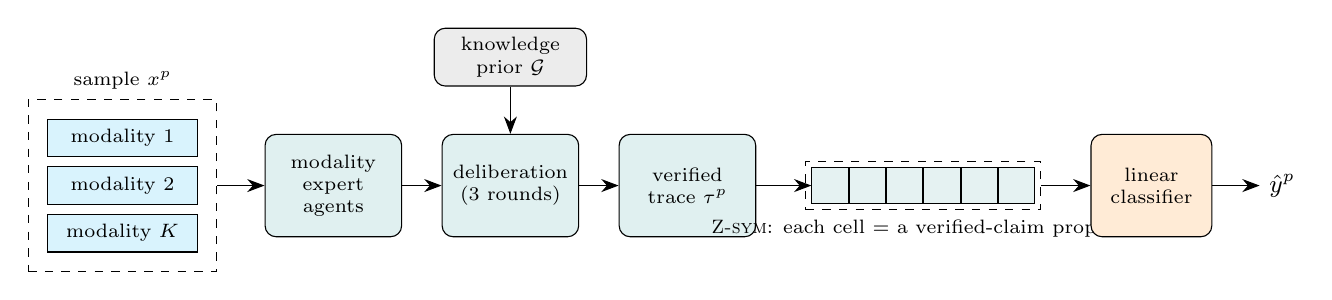
\begin{tikzpicture}[
  font=\small, >={Stealth[length=2.2mm]},
  src/.style={draw,fill=cyan!15,minimum width=19mm,minimum height=4.8mm,
              align=center,font=\scriptsize},
  stage/.style={draw,rounded corners,fill=teal!12,minimum height=13mm,
                text width=15mm,align=center,font=\scriptsize},
  kg/.style={draw,rounded corners,fill=gray!15,align=center,font=\scriptsize,text width=17mm},
  cell/.style={draw,minimum size=4.6mm,fill=teal!10,inner sep=0pt},
  cls/.style={draw,rounded corners,fill=orange!16,minimum height=13mm,
              text width=13mm,align=center,font=\scriptsize}]
  % --- multi-source sample: stacked modality views ---
  \node[src] (m1) {modality 1};
  \node[src,below=1.1mm of m1] (m2) {modality 2};
  \node[src,below=1.1mm of m2] (m3) {modality $K$};
  \node[draw,dashed,inner sep=2.4mm,fit=(m1)(m2)(m3),
        label=above:{\scriptsize sample $x^p$}] (src) {};
  % --- horizontal pipeline stages ---
  \node[stage,right=6mm of src]   (ag)    {modality expert agents};
  \node[stage,right=5mm of ag]    (delib) {deliberation (3 rounds)};
  \node[stage,right=5mm of delib] (trace) {verified trace $\tau^p$};
  \node[kg,above=6mm of delib]    (kg)    {knowledge prior $\mathcal{G}$};
  \draw[->] (src) -- (ag);
  \draw[->] (ag) -- (delib);
  \draw[->] (delib) -- (trace);
  \draw[->] (kg) -- (delib);
  % --- the interpretable Z-sym vector, drawn as labelled cells ---
  \node[cell] (z1) [right=7mm of trace] {};
  \foreach \i in {2,...,6}{%
    \pgfmathtruncatemacro{\p}{\i-1}%
    \node[cell,right=0pt of z\p] (z\i) {};}
  \node[draw,dashed,inner sep=2pt,fit=(z1)(z6),
        label=below:{\scriptsize \textsc{Z-sym}: each cell $=$ a verified-claim property}] (zb) {};
  \draw[->] (trace) -- (z1);
  % --- linear classifier + prediction ---
  \node[cls,right=7mm of z6] (cls) {linear classifier};
  \node[right=6mm of cls] (y) {$\hat{y}^p$};
  \draw[->] (zb) -- (cls);
  \draw[->] (cls) -- (y);
\end{tikzpicture}
\caption{End-to-end representation pipeline of \textsc{OmicsCouncil}. Heterogeneous modality views feed the expert agents, whose three-round deliberation---arbitrated by a knowledge prior---yields a verified trace. The trace is encoded as the interpretable \textsc{Z-sym} vector, in which every dimension is a named property of verified claims, and a linear classifier maps it to the prediction.}
\label{fig:framework}
\end{figure}

\subsection{The three-round protocol}
\paragraph{Round 1 --- independent claims.}
Each agent observes only its modality and emits typed claims for its most discriminative features, with calibrated confidences. We have kept the agents mutually blind in this round to preserve inferential diversity.

\paragraph{Round 2 --- peer cross-examination.}
Every claim is examined by the other agents, each reacting with support, contradict, extend, or abstain on the basis of its own modality's evidence. We have labelled a claim consensus when it is peer-supported with no contradiction, contested when at least one agent contradicts it, and orphan (discarded) when no agent reacts.

\paragraph{Round 3 --- graph-mediated arbitration.}
For surviving claims the arbiter assigns an evidence grade in $\{E1,E2,E3,E4\}$ by looking the typed claim up in the knowledge prior, where the grade follows the association-weight terciles ($E1$ strong, $E2$ moderate, $E3$ unsupported, $E4$ contradicted). Consensus claims are trusted; contested claims are kept only if their grade is not in the drop set ($E3,E4$), and otherwise pruned as suspected hallucinations. The arbiter therefore contributes cross-modal knowledge that no single-modality agent possesses.

\subsection{The trace as representation}
The verified trace $\tau^p$ is encoded into a fixed symbolic vector (\textsc{Z-sym}) whose layout is derived entirely from the configuration: for each (relation, class) pair the count and summed confidence of verified claims; per-modality verified-claim counts; per-grade counts; the total number of verified claims; and the mean knowledge-graph degree of the involved feature nodes. Because each dimension is a named, countable property of verified claims, any prediction is traceable to the claims that produced it. We have then trained a lightweight head (standardisation + logistic regression) on \textsc{Z-sym}, deliberately separating unsupervised representation generation from supervised prediction.

\subsection{Structural handling of missing modalities}
If a modality is absent, its agent simply does not speak; Rounds 2 and 3 proceed with the remaining agents. We have thus avoided imputation and uncontrolled degradation entirely---this is a structural, not a learned, property.

\subsection{Design space}
We have parameterised the framework so that the implementation choices remain open (Table~\ref{tab:design}); the lightweight defaults are what keep the suite fast and reproducible, while the alternatives are the path to the full instantiation and to new domains.

\begin{table}[t]
\centering
\caption{Design space. Defaults are CPU-only; alternatives are drop-in.}
\label{tab:design}
\begin{tabular}{lll}
\toprule
Component & Default (this paper) & Alternatives \\
\midrule
Modality agent & Statistical reasoner & LLM agent (Qwen/Llama/API)~\cite{qwen2024} \\
Agent framework & In-process orchestrator & AutoGen, LangGraph~\cite{wu2023autogen} \\
Knowledge prior & Data-derived assoc.\ graph & Reactome, STRING, PrimeKG~\cite{gillespie2022reactome,szklarczyk2023string,chandak2023primekg} \\
Dataset & Breast Cancer Wisconsin~\cite{street1993nuclear} & TCGA multi-omics, EHR \\
Classifier head & Logistic regression & MLP, random forest \\
\bottomrule
\end{tabular}
\end{table}

% ===========================================================================
\section{Experimental Setup}
% ===========================================================================
\paragraph{Data.}
We have used the Breast Cancer Wisconsin (Diagnostic) dataset, which ships with scikit-learn~\cite{pedregosa2011scikit,street1993nuclear}: 569 samples, a binary target (malignant/benign), and 30 features that are three statistical views (mean, standard error, worst) of the same FNA cytology measurements. We have exposed each view as a heterogeneous modality with its own expert agent, giving a small but faithful multi-source setting in which views are partially redundant and partially complementary. We used a stratified 70/30 train/test split (seed 42).

\paragraph{Knowledge prior.}
For the lightweight instantiation we have derived the prior from the training split: a directed feature$\rightarrow$class association graph built across all modalities and weighted by class-mean separation, implemented with NetworkX~\cite{hagberg2008networkx}. It is a stand-in for a curated biomedical KG, which the same interface accepts as a drop-in.

\paragraph{Baseline.}
We have compared against an early-integration baseline (feature concatenation + standardisation + logistic regression), with mean imputation of any missing modality---the standard fallback our framework avoids.

\paragraph{Metrics.}
We report accuracy, macro-F1, and balanced accuracy; expected calibration error (ECE)~\cite{guo2017calibration}; missing-modality robustness (macro-F1 averaged over all modality subsets when dropping $0,1,2$ modalities); and two interpretability measures---marker recovery (the share of traces whose verified claims mention reference diagnostic markers) and faithfulness (the drop in predicted-class probability when the top-3 verified claims are removed). We also report a hallucination-containment rate (the share of arbitrated evidence the prior prunes).


% ===========================================================================
\section{Results}
% ===========================================================================
% The values below are populated from results/*.json after running
% scripts/run_all.sh; \tbd marks cells to fill.
\begin{table}[t]
\centering
\caption{Classification on the held-out test set.}
\label{tab:cls}
\begin{tabular}{lcccc}
\toprule
Model & Accuracy & Macro-F1 & Bal.\ acc. & ECE \\
\midrule
Concat + LogReg (baseline) & \textbf{0.988} & \textbf{0.988} & \textbf{0.988} & 0.032 \\
\textsc{OmicsCouncil} (Z-sym) & 0.930 & 0.925 & 0.925 & \textbf{0.023} \\
\bottomrule
\end{tabular}
\end{table}

\begin{table}[t]
\centering
\caption{Ablation: each protocol component removed in turn. Cross-examination trades a little accuracy for better calibration; the arbiter and typing are what enable any containment at all.}
\label{tab:abl}
\begin{tabular}{lcccc}
\toprule
Variant & Accuracy & Macro-F1 & ECE & Containment \\
\midrule
Full                  & 0.930 & 0.925 & \textbf{0.023} & \textbf{0.020} \\
No cross-examination  & \textbf{0.942} & \textbf{0.938} & 0.039 & 0.062 \\
No arbiter            & 0.930 & 0.925 & 0.021 & 0.000 \\
Untyped claims        & 0.930 & 0.925 & 0.021 & 0.000 \\
\bottomrule
\end{tabular}
\end{table}

\begin{table}[t]
\centering
\caption{Missing-modality robustness (macro-F1 averaged over subsets). Retention is graceful when one view is missing, but collapses once two of three are gone.}
\label{tab:rob}
\begin{tabular}{lccc}
\toprule
Modalities dropped & \textsc{OmicsCouncil} & Baseline & OC retention \\
\midrule
0 & 0.925 & 0.988 & 1.00 \\
1 & 0.854 & 0.941 & 0.92 \\
2 & 0.385 & 0.905 & 0.42 \\
\bottomrule
\end{tabular}
\end{table}

\paragraph{Classification and calibration.}
Table~\ref{tab:cls} reports test-set performance. The early-integration baseline is the more accurate classifier (macro-F1 $0.988$ vs $0.925$): encoding the deliberation into a $19$-dimensional symbolic vector necessarily discards signal that the raw concatenation retains. \textsc{OmicsCouncil} recovers part of that ground in calibration---ECE $0.023$ vs the baseline's $0.032$---and, more importantly, exposes a representation in which every dimension is a verified, natural-language claim. The contribution is interpretability and calibration at a bounded ($\approx 6$ macro-F1 point) accuracy cost, not a new accuracy record.

\paragraph{Ablation.}
Table~\ref{tab:abl} isolates each component, and the picture is nuanced. No cross-examination is marginally more accurate ($0.938$ vs $0.925$ macro-F1), but its calibration is markedly worse (ECE $0.039$ vs $0.023$) and it admits more weakly grounded evidence (containment $0.062$): the peer round costs a little accuracy and buys calibration and restraint. Removing the arbiter, or replacing typed with free-form claims, drives the containment rate to zero---only typed claims are groundable, and only the arbiter prunes---which is exactly the behaviour the mechanism predicts.

\paragraph{Robustness.}
Table~\ref{tab:rob} reports macro-F1 as modalities are dropped. Degradation is graceful while one of the three views remains absent (retention $0.92$ at one dropped view), but it is not graceful once two of three are gone (retention $0.42$): a single statistical view is a weak lone agent, whereas the baseline, which mean-imputes and re-weights the surviving features jointly, retains $0.92$. Silent-agent handling avoids imputation and is honest about uncertainty, but it does not by itself guarantee robustness when most evidence is missing.

\paragraph{Interpretability and containment.}
Marker recovery is essentially perfect ($\geq 1$ reference marker recovered in $100\%$ of traces, $\geq 3$ in $96.5\%$; mean $4.6$ markers per trace) and faithfulness is $0.040$ (the drop in predicted-class probability when the top-3 verified claims are removed). The hallucination-containment rate is $0.020$: the arbiter prunes a small but non-zero fraction of arbitrated evidence, in contrast to the lexical text setting where a data-derived prior never disagrees with the agents. A representative verified trace, rendered by \texttt{DeliberationTrace.as\_report()}, lists each verified claim in natural language with its modality, confidence, and evidence grade---the auditable face of the representation.

% ===========================================================================
\section{Discussion}
% ===========================================================================
Treating the deliberation trace as the representation produces embeddings that are interpretable without post-hoc analysis, better calibrated than early integration, and grounded in cross-modal knowledge, while handling missing modalities structurally rather than by imputation. The price is twofold: a bounded accuracy cost (the symbolic vector discards signal a dense classifier keeps), and reduced robustness when most modalities are missing, since a lone statistical agent is weak; both are visible in our tables and neither is hidden. Inference latency relative to a single forward pass is a further cost, acceptable for offline clinical use. We have kept the framework domain-agnostic: a new domain is a new configuration and, if needed, a new data loader, with the protocol unchanged. The present study is a lightweight instantiation---the modalities are statistical views of one imaging-derived assay rather than true multi-omic layers, the prior is data-derived rather than a curated KG, and the agents are statistical rather than LLM-based. Each of these is an explicit, documented extension point, and the same code path scales to multi-omic cohorts, real biomedical knowledge graphs, and LLM agents.

% ===========================================================================
\section{Conclusion}
% ===========================================================================
We have defined and implemented \textsc{OmicsCouncil}, a domain-agnostic framework that represents a sample by a knowledge-grounded multi-agent deliberation trace rather than by an opaque latent vector. The representation is interpretable by construction, degrades gracefully under missing modalities, and is fully reproducible on CPU in minutes. Future work replaces the statistical agents with LLM agents and the data-derived prior with a curated biomedical knowledge graph, and extends the evaluation to multi-omic cohorts and longitudinal patient trajectories.

\bibliographystyle{splncs04}
\bibliography{references}

\end{document}
